% Generated by tex/build_swebok_structure.py from tex/chapters/ch01/02_導入：要求が重要な理由.tex
\section{第01章 ソフトウェア要求}
\noindent\textbf{この資料の主張}

ソフトウェア要求は、単なる「欲しい機能の一覧」ではない。要求は、現実世界の問題を解くためにソフトウェアが満たすべき条件、能力、制約を言葉やモデルで表したものである。要求が曖昧なまま設計・実装・テストへ進むと、後で直す範囲が大きくなる。したがって、要求を「引き出す」「分析する」「仕様として書く」「妥当か確認する」「変化を管理する」という一連の活動として扱うことが重要である。

\MiniBox{この資料の読み方}{専門用語は原則として日本語で示し、必要に応じて英語を括弧内に併記する。英語名は、元資料やツール上の名称を確認したいときの手がかりとして残す。初学者が前提知識なしに読めるように、各節では「何のための概念か」「実務では何を見ればよいか」を重視する。}

\subsection{導入}

\paragraph{全体概要：この章で学ぶこと}

この章は、ソフトウェア開発の最初だけでなく、設計・実装・テスト・保守まで影響する「要求」を扱う。ここでいう要求とは、利用者や顧客の希望だけでなく、業務規則、法令、標準、運用上の制約、性能や安全性の水準、予算や納期の制約まで含み得る。

\SmallHead{到達目標}
この章を読み終えると、次のことができるようになる。
\begin{itemize}
\item 「要求」「機能要求」「非機能要求」「技術制約」「サービス品質制約」を区別できる。
\item 要求をどこから集めるか、どのように引き出すかを説明できる。
\item 要求が曖昧・不完全・矛盾している場合に、何を確認すべきかを説明できる。
\item 要求を文章・受け入れ基準・モデルとして記録する方法の違いを説明できる。
\item 要求の妥当性確認、変更管理、優先順位付け、追跡可能性の役割を説明できる。
\end{itemize}

\SmallHead{学習順序}
初学者は、まず「要求とは何か」と「要求の分類」を押さえる。その後、「要求をどう集めるか」「どう分析するか」「どう書くか」「どう確認するか」「どう変化に対応するか」という流れで読むとよい。

\begin{figure}[htbp]
\centering
\IfFileExists{swebok_structure/CH01.ソフトウェア要求(Software_Requirements)/1.0.導入(Introduction)/assets/fig-ch01-01.png}{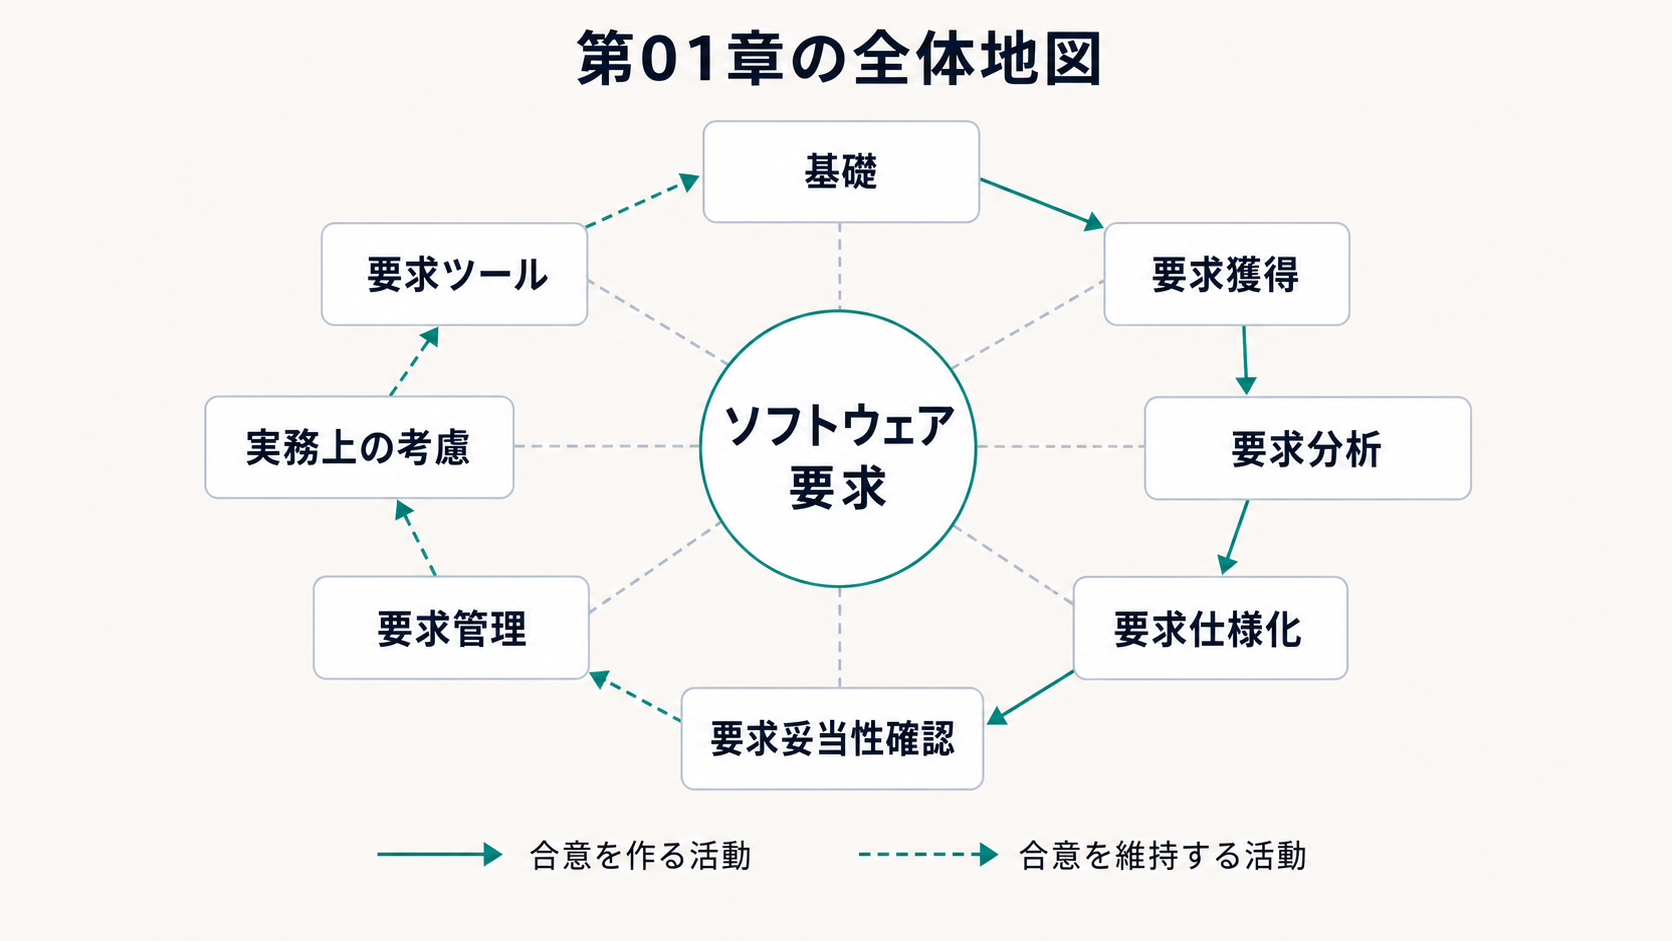
\includegraphics[width=0.96\linewidth]{swebok_structure/CH01.ソフトウェア要求(Software_Requirements)/1.0.導入(Introduction)/assets/fig-ch01-01.png}}{\fbox{\parbox[c][48mm][c]{0.9\linewidth}{\centering 画像生成待ち\\第01章の全体地図}}}
\caption{第01章の全体地図}
\label{fig:ch01-01}
\end{figure}

\subsubsection*{最初に必要な用語}
\addcontentsline{toc}{subsubsection}{最初に必要な用語}

\par\smallskip\noindent\refstepcounter{table}\label{tab:ch01-01}\textbf{表 \thetable: 第01章 ソフトウェア要求 表01}\par\smallskip
\begin{tabularx}{0.97\linewidth}{@{}p{.25\linewidth}X@{}}
\toprule
用語 & 初学者向けの説明 \\
\midrule
\term{ソフトウェア} & プログラムだけでなく、データ、設定、操作手順、関連文書を含むことがある。 \\
\term{要求} & 何かを達成するために満たすべき条件・能力・制約。 \\
\term{利害関係者} & 開発結果に影響を与える、または影響を受ける人・組織。顧客、利用者、運用担当、規制当局など。 \\
\term{システム} & ソフトウェア、ハードウェア、人、手順、設備などが組み合わさって目的を達成するもの。 \\
\term{仕様} & 要求や設計などを、関係者が共有できるように記録したもの。 \\
\term{妥当性確認} & 「これを作れば本当に相手の問題を解決できるか」を確認すること。 \\
\term{追跡可能性} & 要求が設計、コード、テスト、利用者文書などとどうつながるかをたどれること。 \\
\bottomrule
\end{tabularx}

\paragraph{要求が重要な理由}

ソフトウェア要求は、二つの視点から理解する。第一に、要求は「ソフトウェア製品やプロジェクトに対するニーズと制約の表現」である。第二に、要求は「そのニーズと制約を作り、保ち、変化に対応する活動」である。

要求を誤ると、プロジェクトの費用、納期、品質に大きく影響する。ひとつの要求は複数の設計判断を生み、ひとつの設計判断は複数のコード判断を生み、さらに複数のテスト判断につながる。したがって、要求の欠落や誤解が後工程で見つかると、修正範囲が連鎖的に広がる。

現実のプロジェクトで特に多い問題は、\term{不完全性}と\term{曖昧性}である。不完全性とは、必要な要求や詳細が明らかになっていない状態である。曖昧性とは、同じ要求文を複数の意味に解釈できる状態である。どちらも、作ったものが「本来ほしかったもの」とずれる原因になる。

要求文書は、初期開発のためだけではない。保守担当者が後からコードを見ると、コードが「何をしているか」は実行や解析でわかる場合がある。しかし、コードが「何を意図しているか」は要求がなければわかりにくい。欠陥とは、多くの場合、ソフトウェアが意図されたことと実際にしていることの差である。要求は、その意図を長期にわたって伝える役割を持つ。

\MiniBox{重要}{要求活動は、開発の最初に一回だけ行う作業ではない。要求は、プロジェクト開始時に始まり、開発中に洗練され、運用・保守の期間にも参照・変更される。}
